\vspsec
\section{Experiments}\label{sec:results}
\vspsec
Our evaluation aims to answer the following questions: (1) Is adaptation actually changing the model? (2) Does our approach enable fast adaptation to varying dynamics, tasks, and environments, both inside and outside of the training distribution? (3) How does our method's performance compare to that of other methods? (4) How do GrBAL and ReBAL compare? (5) How does meta model-based RL compare to meta model-free RL in terms of sample efficiency and performance for these experiments? (6) Can our method learn to adapt online on a real robot, and if so, how does it perform?
We next present our set-up and results, motivated by these questions. Videos are available online\footnote{Videos available at: \url{https://sites.google.com/berkeley.edu/metaadaptivecontrol}}, and further analysis is provided in the appendix.
We first conduct a comparative evaluation of our algorithm, on a variety of simulated robots using the MuJoCo physics engine~\citep{todorov2012mujoco}. For all of our environments, we model the transition probabilities as Gaussian random variables with mean parameterized by a neural network model (3 hidden layers of 512 units each and ReLU activations) and fixed variance. In this case, maximum likelihood estimation corresponds to minimizing the mean squared error. We now describe the setup of our environments (Fig.~\ref{fig:mujoco-envs}), where each agent requires different types of adaptation to succeed at run-time:

\vspace{-0.1in}
\paragraph{Half-cheetah (HC): disabled joint.} For each rollout during meta-training, we randomly sample a joint to be disabled (i.e., the agent cannot apply torques to that joint). At test time, we evaluate performance in two different situations: disabling a joint unseen during training, and switching between disabled joints during a rollout. The former examines extrapolation to out-of-distribution environments, and the latter tests fast adaptation to changing dynamics.

%\vspace{-0.1in}
\paragraph{HC: sloped terrain.} For each rollout during meta-training, we randomly select an upward or downward slope of low steepness. At test time, we evaluate performance on unseen settings including a gentle upward slope, a steep upward slope, and a steep hill that first goes up and then down.

%\vspace{-0.1in}
\paragraph{HC: pier.} In this experiment, the cheetah runs over a series of blocks that are floating on water. Each block moves up and down when stepped on, and the changes in the dynamics are rapidly changing due to each block having different damping and friction properties. The HC is meta-trained by varying these block properties, and tested on a specific (randomly-selected) configuration of properties.

%\vspace{-0.1in}
\paragraph{Ant: crippled leg.} For each meta-training rollout, we randomly sample a leg to cripple on this quadrupedal robot. This causes unexpected and drastic changes to the underlying dynamics. We evaluate this agent at test time by crippling a leg from outside of the training distribution, as well as transitioning within a rollout from normal operation to having a crippled leg.


In the following sections, we evaluate our model-based meta-RL methods (GrBAL and ReBAL) in comparison to several prior methods:
\begin{itemize}[leftmargin=*]
\item \textbf{Model-free RL (TRPO)}: To evaluate the importance of adaptation, we compare to a model-free RL agent that is trained across environments $\mathcal{E}\sim\rho(\mathcal{E})$ using TRPO~\citep{schulman2015trust}.
\item \textbf{Model-free meta-RL (MAML-RL)}: We compare to a state-of-the-art model-free meta-RL method, MAML-RL~\citep{finn2017maml}.
\item \textbf{Model-based RL (MB)}: Similar to the model-free agent, we also compare to a single model-based RL agent, to evaluate the importance of adaptation. This model is trained using supervised model-error and iterative model bootstrapping. %, and an MPPI planner~\cite{williams15mppi}.
\item \textbf{Model-based RL with dynamic evaluation (MB+DE)}: We compare to an agent trained with model-based RL, as above. However, at test time, the model is adapted by taking a gradient step at each timestep using the past $M$ observations, akin to dynamic evaluation~\citep{krause2017dynamiceval}. This final comparison evaluates the benefit of explicitly training for adaptability.
\end{itemize}

All model-based approaches (MB, MB+DE, GrBAL, and ReBAL) use model bootstrapping, use the same neural network architecture, and use the same planner within experiments: MPPI~\citep{williams15mppi} for the simulated experiments and random shooting (RS)~\citep{nagabandi2017neural} for the real-world experiments.


\begin{wrapfigure}{R}{0.55\textwidth}
\centering
\vspace{-0.1in}
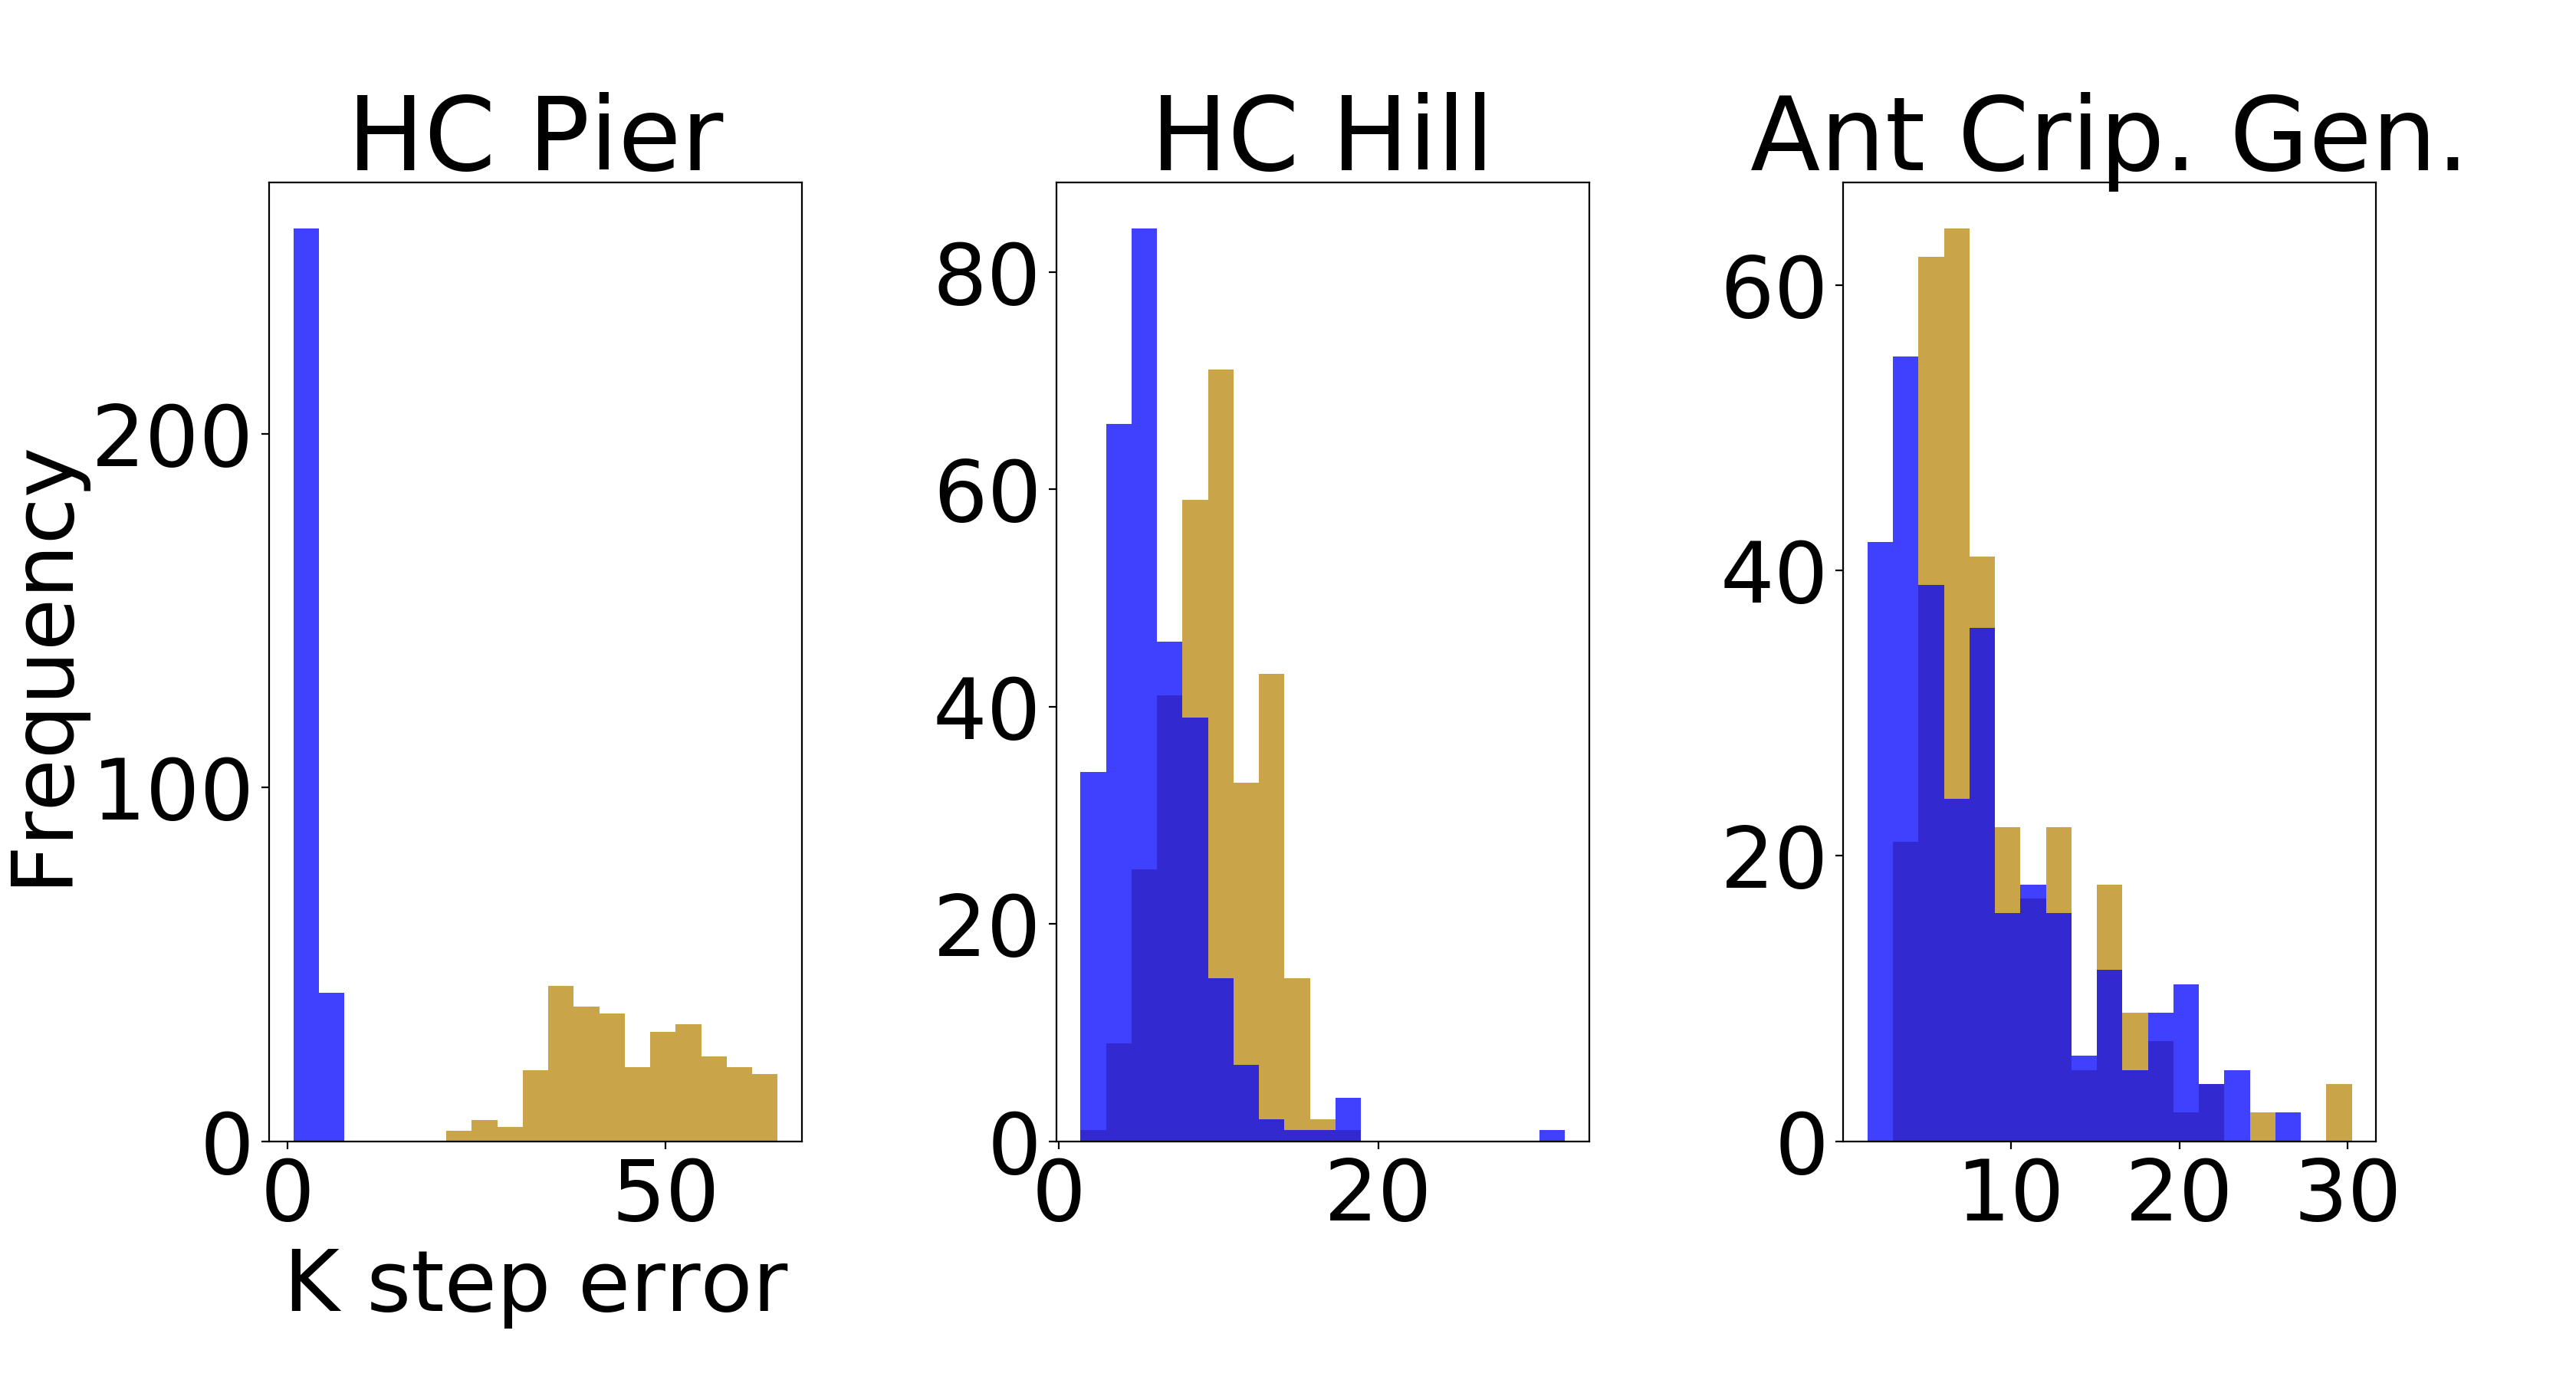
\includegraphics[width=\linewidth]{pictures/hist.png}

\includegraphics[height=0.03\textwidth, width=0.7\linewidth]{pictures/caption_hist.png}
\vspace{-0.3cm}
\caption{\small Histogram of normalized $K$-step model prediction errors of GrBAL, showing the improvement of the post-update model's predictions over the pre-update ones.}
\label{fig:model_errors} 
\vspace{-0.2in}
\end{wrapfigure}
% 
% \vspsubsec
\subsection{Effect of Adaptation}
\vspsubsec
First, we analyze the effect of the model adaptation, and show results from test-time runs on three environments: HC pier, HC sloped terrain with a steep up/down hill, and ant crippled leg with the chosen leg not seen as crippled during training. Figure~\ref{fig:model_errors} displays the distribution shift between the pre-update and post-update model prediction errors of three GrBAL runs, showing that using the past $M$ timesteps to update $\bm{\theta_*}$ (pre) into $\bm{\theta_*'}$ (post) does indeed reduce model error on predicting the following $K$ timesteps.

\subsection{Performance and Meta-training Sample Efficiency}\label{sec:baselines}
\vspsubsec

We first study the sample efficiency of the meta-training process.
Figure~\ref{fig:learning_curves} shows the average return across test environments w.r.t. the amount of data used for meta-training. We (meta-)train the model-free methods (TRPO and MAML-RL) until convergence, using the equivalent of about two days of real-world experience. In contrast, we meta-train the model-based methods (including our approach) using the equivalent of 1.5-3 hours of real-world experience. Our methods result in superior or equivalent performance to the model-free agent that is trained with $1000$ times more data. Our methods also surpass the performance of the non-meta-learned model-based approaches. Finally, our performance closely matches the high asymptotic performance of the model-free meta-RL method for half-cheetah disabled, and achieves a suboptimal performance for ant crippled but, again, it does so with the equivalent of $1000$ times less data. Note that this suboptimality in asymptotic performance is a known issue with model-based methods, and thus an interesting direction for future efforts.
The improvement in sample efficiency from using model-based methods matches prior findings~\citep{deisenroth2011pilco,nagabandi2017neural,thanard}; the most important evaluation, which we discuss in more detail next, is the ability for our method to adapt online to drastic dynamics changes in only a handful of timesteps.

% 
\begin{figure}[H]
\centering
\vspace{-0.1in}
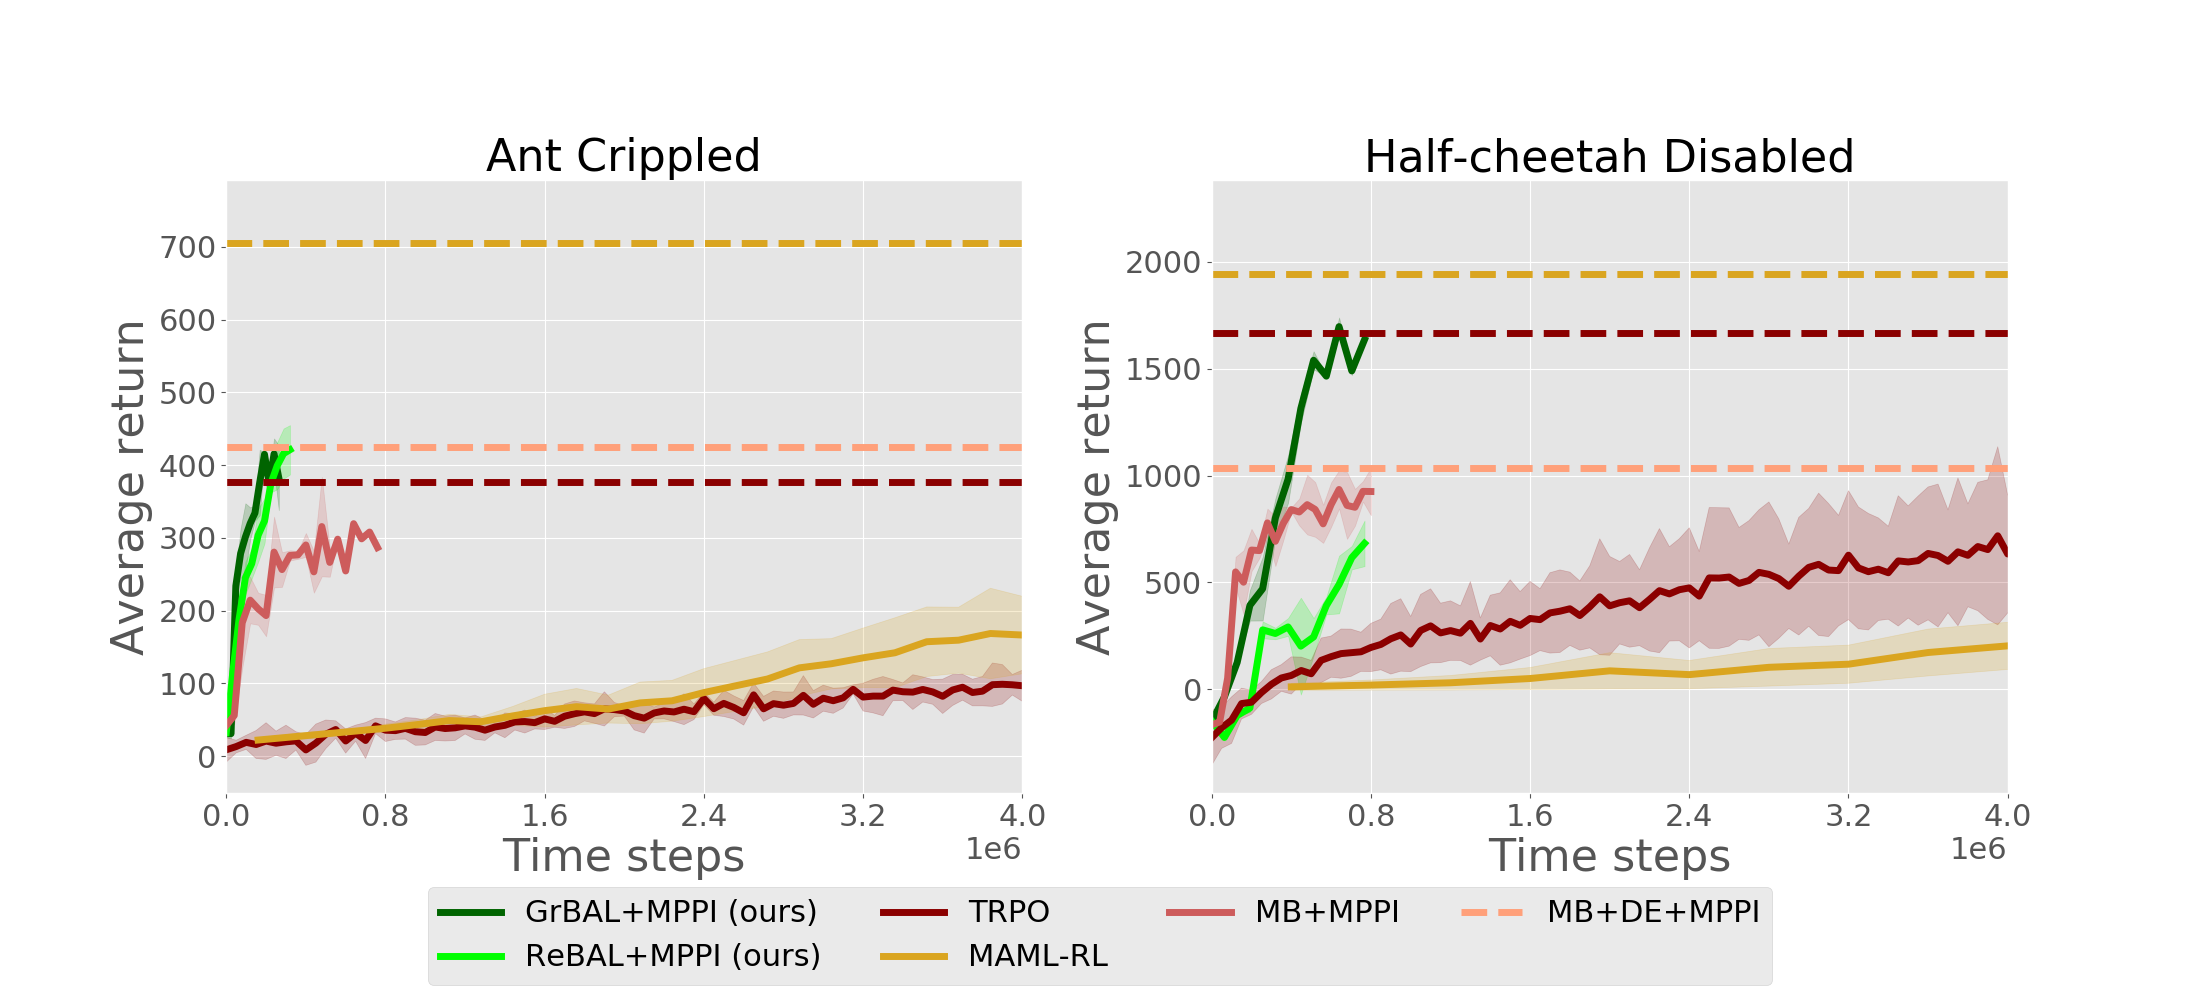
\includegraphics[width=0.9\linewidth]{pictures/sample_efficiency.png}
\vspace{-0.1in}
\caption{\small Compared to model-free RL, model-free meta-RL, and model-based RL methods, our model-based meta-RL methods achieve good performance with 1000$\times$ less data. Dotted lines indicate performance at convergence. For MB+DE+MPPI, we perform dynamic evaluation at test time on the final MB+MPPI model.}
\label{fig:learning_curves}
\vspace{-0.1in}
\end{figure}

\begin{wrapfigure}{R}{0.4\textwidth}
\vspace{-0.4in}
\centering
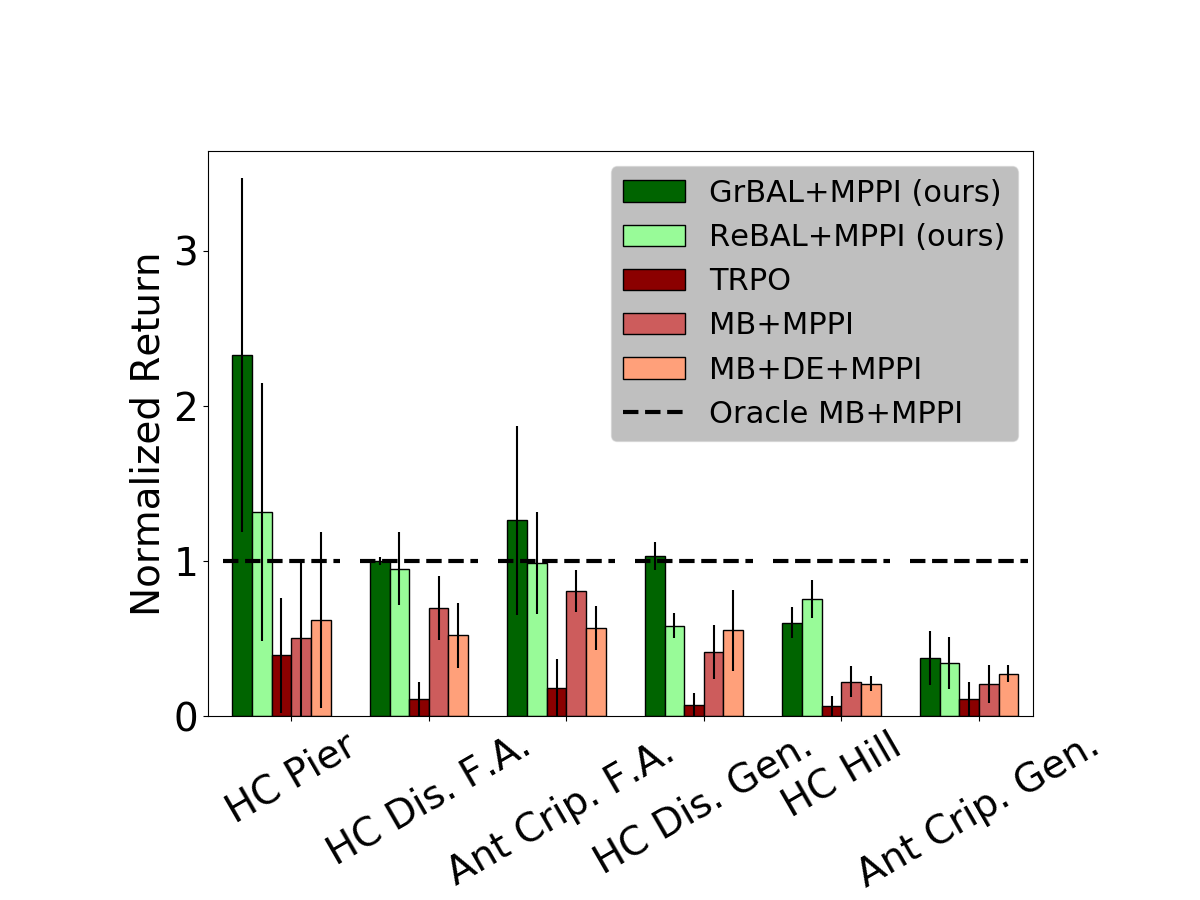
\includegraphics[width=\linewidth]{pictures/simulated_experiments.png}
\caption{\small Simulated results in a variety of dynamic test environments. GrBAL outperforms other methods, even the MB oracle, in all experiments where fast adaptation is necessary. These results highlight the difficulty of training a global model, and the importance of adaptation.
}
\label{fig:sim_exp}
\vspace{-0.1in}
\end{wrapfigure}

\vspsubsec
\subsection{Test-time Performance: Online Adaptation \& Generalization}\label{sec:fast_adapt}
\vspsubsec

In our second comparative evaluation, we evaluate final test time performance both GrBAL and ReBAL in comparison to the aforementioned methods.
In the interest of developing efficient algorithms for real-world applications, we operate all methods in the low data regime for all experiments: the amount of data available (meta-)training is fixed across methods, and roughly corresponds to 1.5-3 hours of real-world experience depending on the domain. We also provide the performance of a MB oracle, which is trained using unlimited data from only the given test environment (rather than needing to generalize to various training environments).

In these experiments, note that all agents were meta-trained on a distribution of tasks/environments (as detailed above), but we then evaluate their adaptation ability on unseen environments at test time. We test the ability of each approach to adapt to sudden changes in the environment, as well as to generalize beyond the training environments. We evaluate the fast adaptation (F.A.) component on the HC disabled joint, ant crippled leg, and the HC pier. On the first two, we cause a joint/leg of the robot to malfunction in the middle of a rollout. We evaluate the generalization component also on the tasks of HC disabled joint and ant crippled leg, but this time, the leg/joint that malfunctions has not been seen as crippled during training. The last environment that we test generalization on is the HC slopped terrain for a hill, where the agent has to run up and down a steep slope, which is outside of the gentle slopes that it experienced during training. The results, shown in Fig.~\ref{fig:sim_exp}, show returns that are normalized such that the MB oracle achieves a return of 1.

In all experiments, due to low quantity of training data, TRPO performs poorly. Although MB+DE achieves better generalization than MB, the slow nature of its adaptation causes it to fall behind MB in the environments that require fast adaptation. On the other hand, our approach surpasses the other approaches in all of the experiments. In fact, in the HC pier and the fast adaptation of ant environments, our approach surpasses the model-based oracle. This result showcases the importance of adaptation in stochastic environments, where even a model trained with a lot of data cannot be robust to unexpected occurrences or disturbances. ReBAL displays its strengths on scenarios where longer sequential inputs allow it to better asses current environment settings, but overall, GrBAL seems to perform better for both generalization and fast adaptation.

\vspsubsec
\subsection{Real-World Results}
\vspsubsec
To test our meta model-based RL method's sample efficiency, as well as its ability to perform fast and effective online adaptation, we applied GrBAL to a real legged millirobot, comparing it to model-based RL (MB) and model-based RL with dynamic evaluation (MB+DE). Due to the cost of running real robot experiments, we chose the better performing method (i.e., GrBAL) to evaluate on the real robot.
This small 6-legged robot, as shown in Fig.~1 and Fig.~\ref{fig:mujoco-envs}, presents a modeling and control challenge in the form of highly stochastic and dynamic movement. This robot is an excellent candidate for online adaptation for many reasons: the rapid manufacturing techniques and numerous custom-design steps used to construct this robot make it impossible to reproduce the same dynamics each time, its linkages and other body parts deteriorate over time, and it moves very quickly and dynamically with 

The state space of the robot is a 24-dimensional vector, including center of mass positions and velocities, center of mass pose and angular velocities, back-EMF readings of motors, encoder readings of leg motor angles and velocities, and battery voltage. We define the action space to be velocity setpoints of the rotating legs. The action space has a dimension of two, since one motor on each side is coupled to all three of the legs on that side. All experiments are conducted in a motion capture room. Computation is done on an external computer, and the velocity setpoints are streamed over radio at 10 Hz to be executed by a PID controller on the microcontroller on-board of the robot.

We meta-train a dynamics model for this robot using the meta-objective described in Equation~\ref{eq:metaobj}, and we train it to adapt on entirely real-world data from three different training terrains: carpet, styrofoam, and turf. We collect approximately 30 minutes of data from each of the three training terrains. This data was entirely collected using a random policy, in conjunction with a safety policy, whose sole purpose was to prevent the robot from exiting the area of interest.

Our first group of results (Table~\ref{tbl:roach_table}) show that, when data from a random policy is used to train a dynamics model, both a model trained with a standard supervised learning objective (MB) and a GrBAL model achieve comparable performance for executing desired trajectories on terrains from the training distribution.

Next, we test the performance of our method on what it is intended for: fast online adaptation of the learned model to enable successful execution of new, changing, or out-of-distribution environments at test time. Similar to the comparisons above, we compare GrBAL to a model-based method (MB) that involves neither meta-training nor online adaptation, as well as a dynamic evaluation method that involves online adaptation of that MB model (MB+DE).
Our results (Fig.~6) demonstrate that GrBAL substantially outperforms MB and MB+DE, and, unlike MB and MB+DE, and that GrBAL can quickly 1) adapt online to a missing leg, 2) adjust to novel terrains and slopes, 3) account for miscalibration or errors in pose estimation, and 4) compensate for pulling payloads.
None of these environments were seen during training time, but the agent's ability to learn how to learn enables it to quickly leverage its prior knowledge and fine-tune to adapt to new environments online. Furthermore, the poor performance of the MB and MB+DE baselines demonstrate not only the need for adaptation, but also the importance of good initial parameters to adapt from (in this case, meta-learned parameters).
The qualitative results of these experiments in Fig.~\ref{fig:roach_test} show that the robot is able to use our method to adapt online and effectively follow the target trajectories, even in the presence of new environments and unexpected perturbations at test time.

bounding-style gaits; hence, its dynamics are strongly dependent on the terrain or environment at hand.
\begin{figure*}
\noindent
\begin{minipage}[t]{0.475\textwidth}
\centering
\vspace{-0.1in}
\begin{table}[H]

\centering
\footnotesize
\resizebox{\linewidth}{!}{%
\begin{tabular}{|ll||l|l|l|l|}
\hline
                                                 &       & Left & Str &  Z-z& F-8 \\ \hline \hline
\multicolumn{1}{|l|}{\!\!Carpet\!}    & GrBAL & 4.07 & 3.26     & 7.08    & 5.28     \\ \cline{2-6} 
\multicolumn{1}{|l|}{}                           & MB    & 3.94 & 3.26     & 6.56    & 5.21     \\ \hline
\multicolumn{1}{|l|}{\!\!Styrofoam\!} & GrBAL & 3.90 & 3.75     & 7.55    & 6.01     \\ \cline{2-6} 
\multicolumn{1}{|l|}{}                           & MB    & 4.09 & 4.06     & 7.48    & 6.54     \\ \hline
\multicolumn{1}{|l|}{\!\!Turf}      & GrBAL & 1.99 & 1.65     & 2.79    & 3.40     \\ \cline{2-6} 
\multicolumn{1}{|l|}{}                           & MB    & 1.87 & 1.69     & 3.52    & 2.61     \\ \hline
\end{tabular}%
}
\caption{\small Trajectory following costs for real-world GrBAL and MB results when tested on three terrains that were seen during training. Tested here for left turn (Left), straight line (Str), zig-zag (Z-z), and figure-8 shapes (F-8). The methods perform comparably, indicating that online adaptation is not needed in the training terrains, but including it is not detrimental.
\label{tbl:roach_table}
}
\end{table}
% \vspace{-0.1in}
\end{minipage}
\noindent
\hspace{0.1cm}
\begin{minipage}[t]{0.475\textwidth}
\noindent
\centering
\vspace{-0.1in}
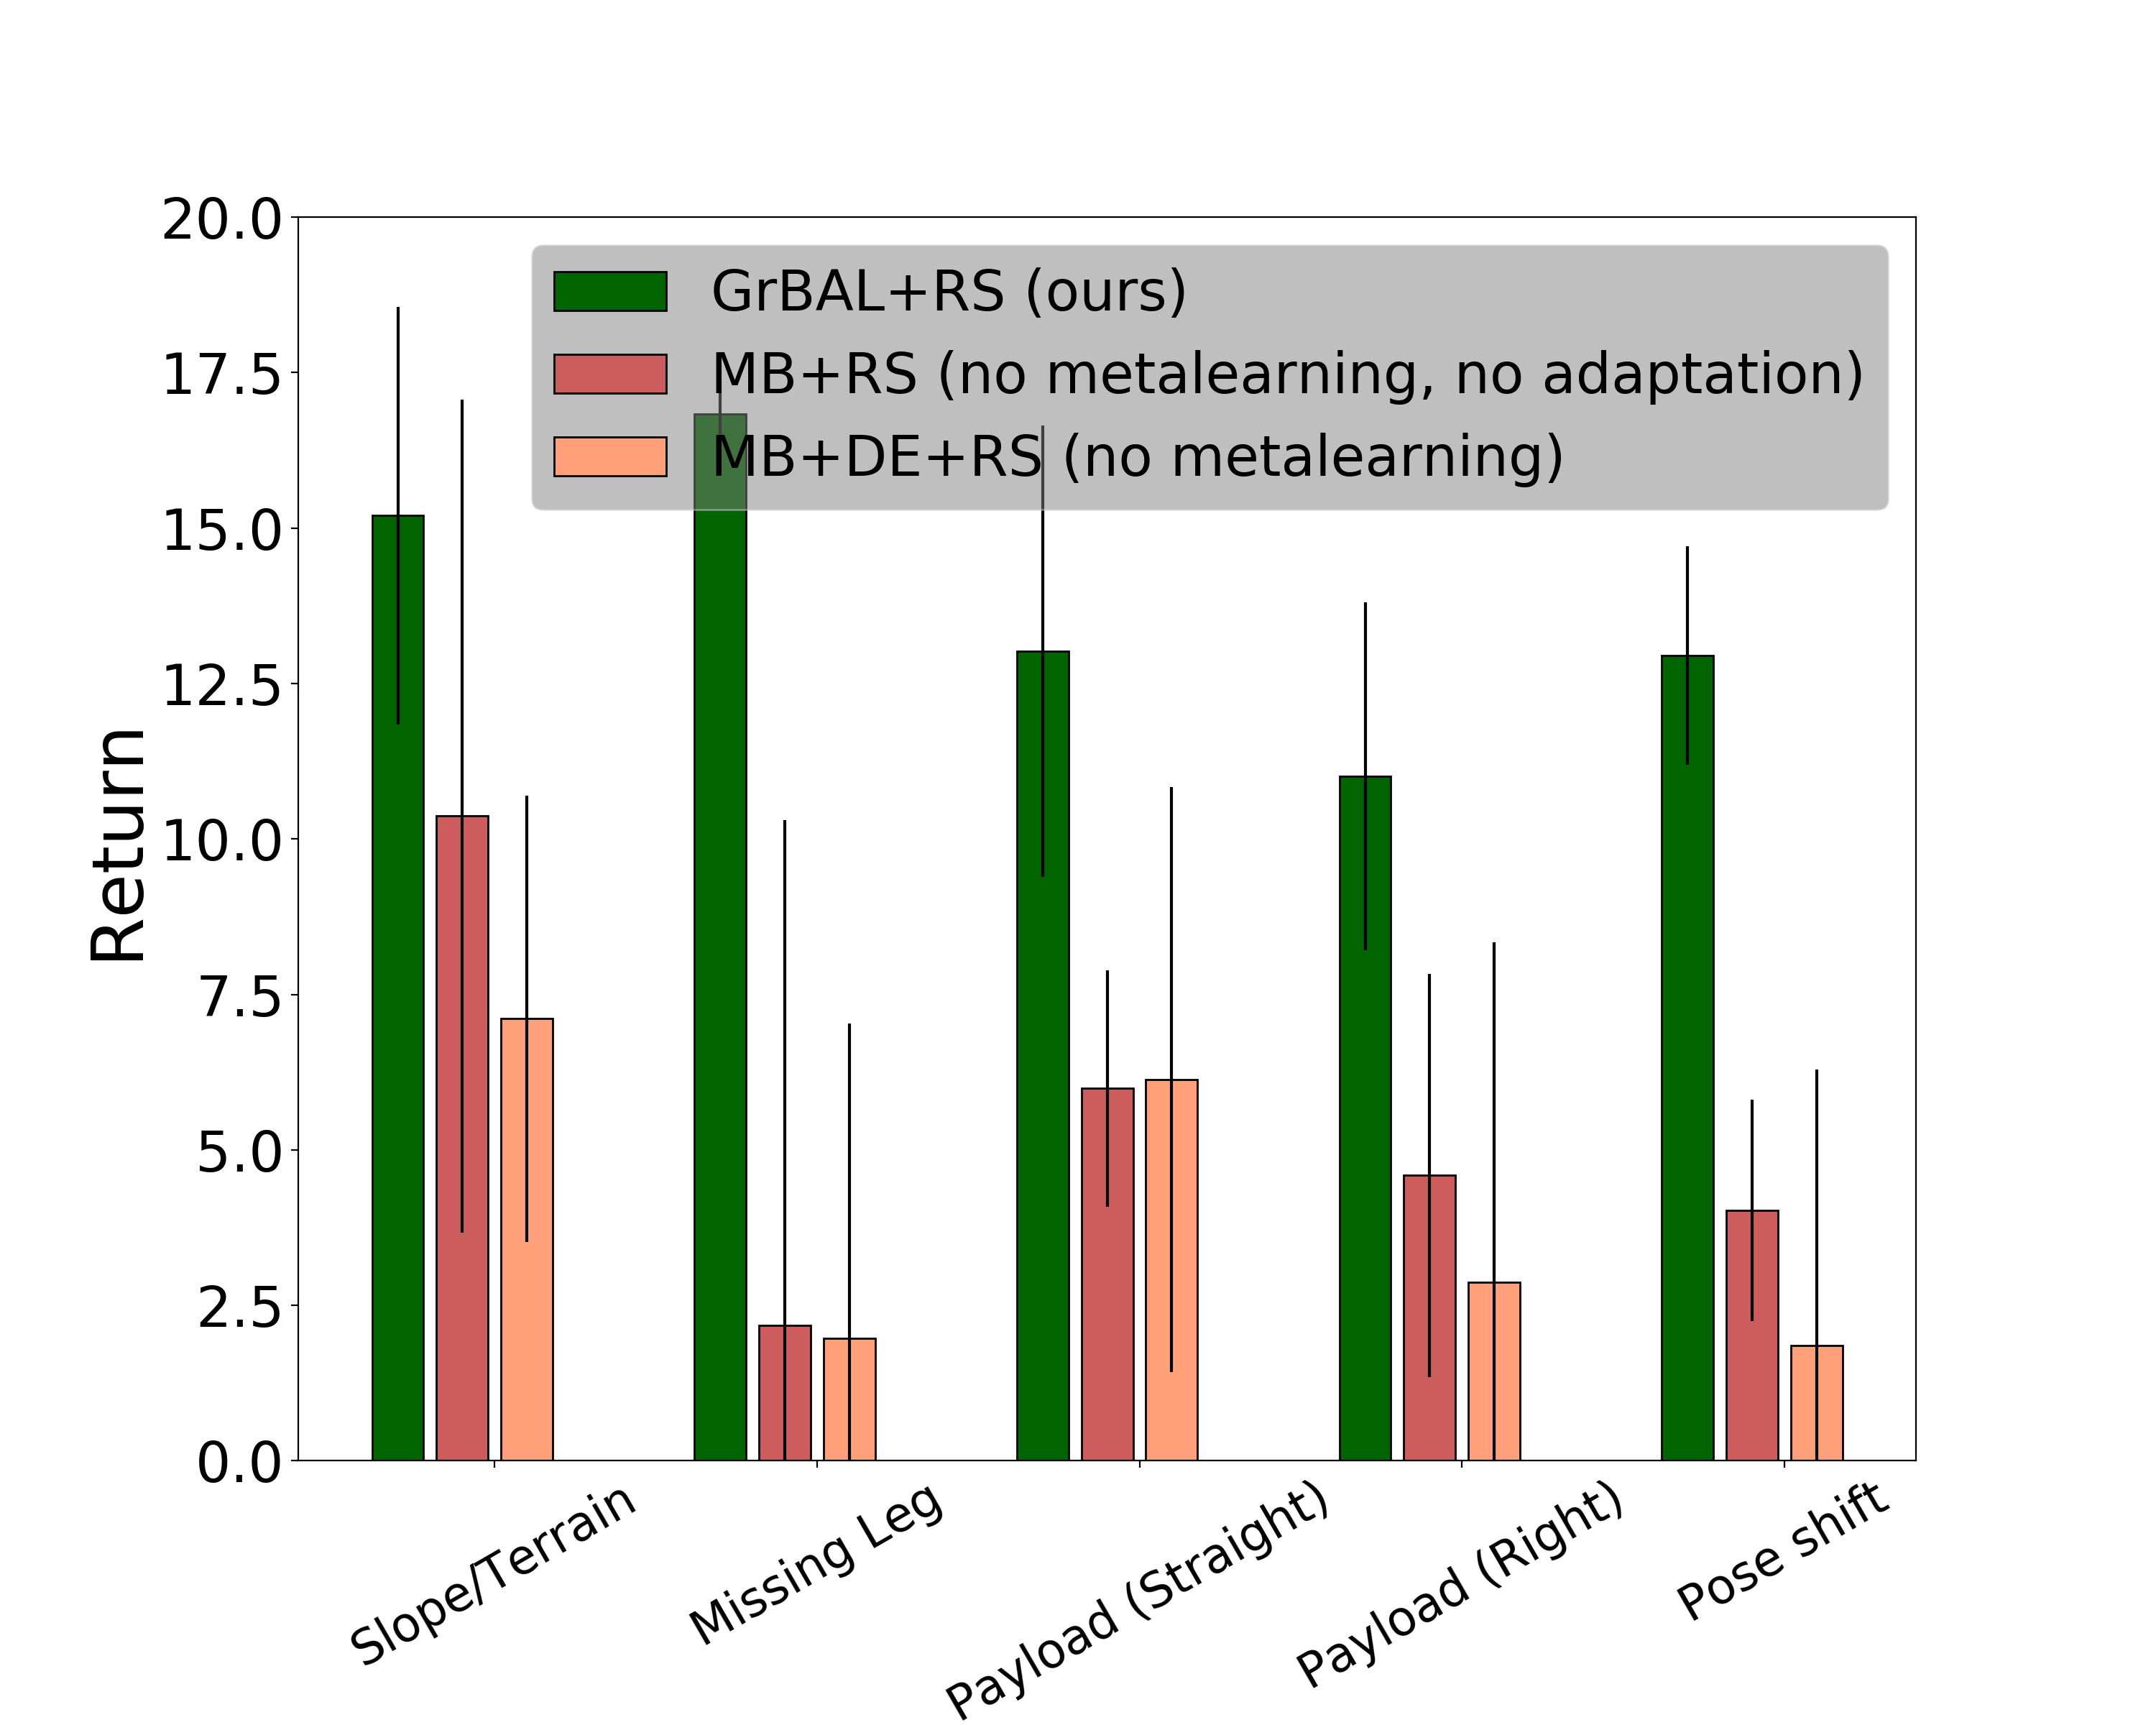
\includegraphics[width=\linewidth]{pictures/roach_testTasks.png}
\label{fig:roach_bars}
\vspace{-0.7cm}
\caption{\small GrBAL clearly outperforms both MB and MB+DE, when tested on environments that (1) require online adaptation, and/or (2) were never seen during training.}
\end{minipage}
\vspace{-0.2 in}
\end{figure*}

\begin{figure}[H]
\centering
\vspace{-0.1in}
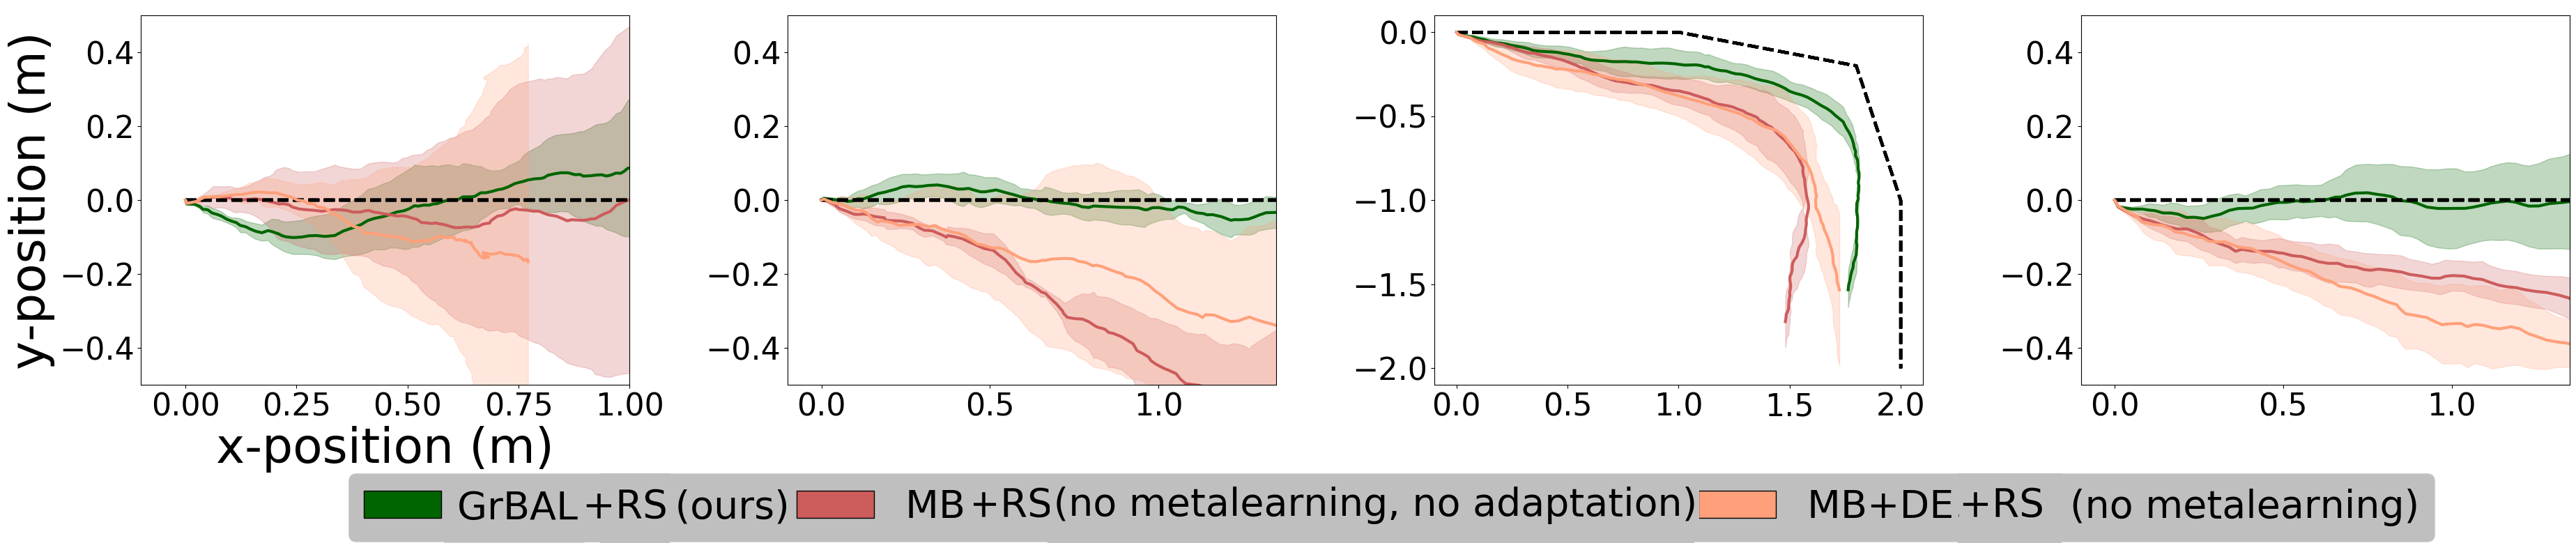
\includegraphics[width=\linewidth]{pictures/paths.png}
\caption{\small The dotted black line indicates the desired trajectory in the $xy$ plane. By effectively adapting online, our method prevents drift from a missing leg, prevents sliding sideways down a slope, accounts for pose miscalibration errors, and adjusts to pulling payloads (left to right). Note that none of these tasks/environments were seen during training time, and they require fast and effective online adaptation for success.}
\label{fig:roach_test}
\end{figure}